\chapter{}
\begin{thought}
Monique brought up the file on the laptop that listed the potential ``injuries.'' She then
accessed the random number generator. She hoped for something good as she instructed it to
generate a single random number between one and one hundred. She hit the ``enter'' key.
\end{thought}

``29''

\begin{thought}
She looked at the list, and found 29 on it. ``Elbow- left.'' Not bad, but not as big as she'd
hoped for.
\end{thought}

``Doctor, your patient has fractured her left elbow.''

``Well,'' I said, playing along, ``we need to get it reduced and immobilized right away. I'll
prepare the casting room.''

I headed to the bathroom and laid out the drop cloth, three inch stockinette, padding and
two and three inch plaster bandages. Monique had hobbled in after me and watched as I filled the
plastic basin with warm water.

``Good! More plaster.'' she said.

``Sure. It will match that long leg cast you already have. To be honest, that cast looks so
good, I don't want to take it off just yet.'' I sat on the edge of the tub and motioned for her
to sit on the commode.

``I don't either,'' she said as she carefully sat down. I slipped the stockinette up her arm
all the way to the shoulder, and made sure to leave some extra bunched up at the top. I made a
diagonal cut for her thumb, and then cut it off near her fingertips.

\begin{thought}
The stockinette felt great as Quinn slid it up her arm, it was smooth, soft and cool from
the air conditioned room. Monique watched intently as he made the cuts at her hand, and then
began wrapping one inch padding around her hand and wrist. When that was covered, he started at
her armpit with three inch padding, working downward. He made an extra turn at the elbow, which
she knew from experience was to pad the bones that were close to the skin.

When the padding was finished, he put on his gloves and unwrapped a roll of two inch
plaster bandage. He started at the wrist, and worked around the hand, taking care to mold the
cast well around the thumb opening and fingers. He folded back the padding and stockinette and
used another roll to anchor it, and then worked up her forearm. She knew she shouldn't move her
hand yet, but the cast looked as though she would have good movement of her thumb and fingers
when the cast was dry.

He used three inch tape to finish the cast, and he worked from the armpit downward to the
forearm. She also knew why he did this: by wrapping from the larger part of the extremity to the
smaller, it allowed each turn of the plaster to keep the previous turn from bunching up. This
kept the cast nice and smooth, as well as eliminating pressure spots inside the cast. The feel
of his hands wrapping and molding the cast, and the smell of the wet plaster were as pleasing as
watching him work.

By the time he was finished wrapping the cast, her hand and wrist were already warm from
the setting plaster. He then began buffing out the surface of the setting plaster with his hands
until it was perfectly smooth. The cast looked great- it was well formed, and thick enough to do
the job and look right, but not bulky anywhere. He also brought the cast up very high on her
arm. She couldn't tell for sure, but she wondered if it would dig in to her armpit if she
lowered her arm all the way.
\end{thought}

``Wow, it comes up really high.'' She said.

``Yes,'' I answered. We want to make sure the elbow is properly immobilized.

I held her arm for a short while longer, until I was certain that the plaster had set
enough to allow her to lower her arm. I gently lowered her arm until it rested against her body.

``How does it feel? Is it digging into your armpit?'' I asked.

``No, it actually feels great,'' Monique said. She wiggled her fingers and thumb. ``Nice
mobility of the hand, too. Excellent work, doctor!''

``Thank you, you're an outstanding patient.''

She leaned forward, and used her uncasted right arm to help herself stand up. She stepped
out of the bathroom and over near the bed. It took her a few steps to get used to balancing on
the leg cast with her arm now immobilized, too.

By this time, it was getting rather late, so we sat on the bed to watch some television
while the cast dried a bit further. Monique snuggled into me on my left, and before long, we
fell asleep.

We woke up Saturday morning still wearing our clothes from the previous day. We took turns
bathing and getting dressed. Of course, it took Monique a bit longer, and due to her casts, she
was forced to give herself a sponge bath as opposed to my hot shower. The sight of her emerging
from the bathroom, nude except for her plaster long arm and long leg casts was quite a sight to
see. I took in the view, and smiled. She would be beautiful covered in mud, but the plaster
hugging the lines of her arm and leg made her absolutely stunning.

``Hello, anyone in there?'' she asked, waving her free hand in front of my eyes.

I smiled and chuckled. ``Hey,'' I said. ``Can I help it if I find you beautiful?''

She smiled and hobbled up to me. I stood up and embraced her, my hands exploring the smooth
skin on her back. We melted into a nice long kiss, and a short time later, we found ourselves
needing to bathe again.

After we'd repeated the bathing process, she picked out clothes for the day, and I helped
her get dressed. She'd been able to undress herself, but getting dressed presented her with a
few challenges. She'd picked out a red tank top and denim shorts for the day. Once we were both
dressed, she began brushing out her hair and asked ``Where are we going today? After we eat, of
course- I'm hungry.''

``I think we'll head back to that area near the art store. It looked kind of interesting to
me. What do you think?''

``Sounds good, let's get going.''

I set up the wheelchair for her, and wheeled her out to the elevator. I used the key card
to call the elevator, and we were soon out the door and on our way. We didn't even see a single
person as we left the hotel.

We stopped at a small restaurant for a late breakfast. Most people were eating lunch by
this time, but we were still able to get a not good, but edible meal. Afterwards, we headed
across town to the Broad Ripple area. Just as it had been the day before, it looked like a
long-established area. I hesitate to say old, as everything was very well-kept. Driving through
the area looking for a parking place took a bit of time, as the traffic moved slow as there was
all manner of pedestrian traffic, and a lot of it. We saw cyclists, joggers, rollerbladers,
joggers, and people just walking around in small groups.

We found a parking place, and I started to get out the wheelchair. Monique stopped me.

``How about we just go on foot for now? If walking starts to get uncomfortable, we'll come
back for the chair.'' I agreed, and helped her out of the truck. I slung a small backpack that
I'd loaded up with art supplies over my shoulder. We headed towards a coffee shop we'd just
passed that offered outdoor seating. Monique took a seat near the sidewalk while I went in to
get our drinks.

\begin{thought}
The sun warmed Monique's face as she took in the sights. People walking, jogging, biking
and skating by. Several looked over at her, sitting there by herself. She smiled at the ones who
looked, especially the few who took a bit more than a casual glance. It didn't take too long
before it dawned on her that there seemed to be more people on bicycles and rollerblades than
she would have expected. Her arm and leg felt good in the casts. The walk from the truck to the
coffee shop had been the longest she'd walked in this leg cast, but Quinn had padded it nearly
perfectly, and she couldn't feel any hot spots from rubbing. The arm cast was heavy, and she
wondered if she might regret not having a sling before the day was over, but for now, everything
felt fine. No- better than fine. It was a beautiful day, she'd started the day off in casts,
moved on to lovemaking, and now was going out for a day in her casts with Quinn. Tonight would
probably bring another cast, and she could look forward to more of this tomorrow!
\end{thought}

``Is this seat taken?'' I asked as I returned. I handed Monique her coffee, and sat down
across from her. We sat and talked awhile, and then we got up and headed down the sidewalk,
window shopping at the small stores, going in any that caught our interest. I mentioned to
Monique that there seemed to be a lot of people on bikes and rollerblades, and they seemed to be
dressed for exercise rather than dressed just to be out. She told me that she'd had the same
thought.

As we moved Eastward along the street, many people turned to take looks at the beautiful
woman in the big casts walking along. In one of the shops, a clerk asked Monique what had
happened to her. Always thinking on her feet, she answered.

``I fell while rollerblading.''

``Wow,'' said the clerk. ``That must have been one heck of a fall!''

``Well,'' she said, ``I was moving pretty fast, and ran off the pavement. There was a hole
just off the road, and when my foot dropped into it, my leg bent just the wrong way and broke.
When I fell, I landed on my arm wrong.''

``Did it happen on the Monon?'' He asked, pointing his thumb to the East.

Monique didn't know what ``The Monon'' was, so she answered with ``No, this happened back
home, in Kentucky.

We said our goodbyes, and continued Eastward down the street. In a short time, we learned
exactly what ``The Monon'' was: It was a paved trail that had been built on an old railroad bed.
The trains that had once run through the area had been a part of the Monon line, and when the
rails were removed for the pedestrian trail, they had named it the Monon rail trail. The trail
had quite a few people on it, and we quickly learned where the cyclists and bladers had been
going- they were all headed to this trail. Many people were on bikes or on roller blades. There
were also a lot of joggers, and many people walking alone and in small groups. I turned to
Monique.

``Want to give it a try?'' I asked.

``Sure!'' she said. ``But I don't think I want to get back on my blades for a while,'' she
added with her mischievous smile.

The trail was quite beautiful. It was easy to see why so many people were using it on a
beautiful Summer Saturday. Trees lined most of the way. At the places where it crossed roads,
the intersections were well marked, and it seemed that the car traffic was very careful of the
people.

A small road ran beside the trail at one point, and we noticed a hiking shop across the
street. Monique pointed it out and suggested we go check it out, so we left the trail, and
crossed the street to the shop.

The hiking shop was a converted craftsman style home, and though it had been remodeled to
serve as a store, the quarters were cramped. The walls were covered with hiking boots and packs.
Clothes adorned a room that appeared to have once been a kitchen. A large semicircular glass
display case had been set up in what had once been the living room, and the cash register and
clerk were there. The clerk greeted us as we walked in, and took the longer than usual look at
Monique that we'd long ago learned to expect.

Monique walked over to the boots and began looking through the different styles.

``We should take a hiking trip sometime.'' She said. ``My father used to go out into the woods
to do landscapes, and I'd go with him whenever I could.''

Keeping up the charade, I replied with ``We can go as soon as you get healed up.''

Monique sighed. ``This really sucks. I hate getting hurt and having to lug these casts
around. Especially since it's summertime, and I can't do much.'' She was definitely putting on a
show for the clerk, who finally could hold her curiosity no longer.

``If you don't mind me asking, what happened to you?'' She said.

``I took a fall on my 'blades. Seeing all of these people out here on theirs sure doesn't
make me feel any better, either.'' She picked up a pair of boots. ``May I try these on? Well,
may
I try the right one on, anyway?''

``Certainly!'' the clerk relied. She pulled up a chair and handed her one of the cheap sheer
foot socks that were kept for customers who weren't wearing socks. I helped Monique ease down
into the chair, left leg sticking out in front of her. I slipped off her sandal, and helped her
get her right foot into the boot. I laced it up, and helped her to stand. She walked around the
store a bit.

``How do they feel?'' the clerk asked without thinking.

Monique didn't miss the opportunity to, once again, call attention to her casts. ``Well, the
right one feels great, but the left is a real problem,'' she said with a smile. The clerk turned
a bit red with embarrassment as she apologized. Monique turned to me.

``It feels really good. A hiking trip would be awesome, and it would be a great way to get
the strength back in my leg once I get this stupid cast off.''

I smiled at her. ``Are you saying you want the boots?''

``Yes''

I turned to the clerk. ``Ring them up, please.''

With me carrying our purchase, we left the store, and headed further up the trail. We'd
noticed a mile marker along the way, and wondered how far this trail actually went. We stopped a
guy who had been having himself a nice gawk at Monique and asked him how long the trail was. As
it turned out, it went about five miles north of where we'd entered it, and a few miles south,
as well.

We continued along the trail for another mile, and found an old iron bridge sporting a
fresh looking coat of red paint. Monique looked ready for a rest, so we sat on one of the shaded
benches at the side of the trail near the bridge. Monique scooted close to me, and I put my arm
around her. We sat for awhile without talking, as we often did. The silence was never
uncomfortable between us. After a while, she broke the silence.

``Will you really go hiking with me?'' she asked.

``Sure''

``Where should we go?'' was her next question.

``Monique, so far, I've been the one deciding where we go all the time. Since this one is
your idea, I'll let you decide where we go.''

``There's something that bothers me about that,'' she said. When I asked her what, she told
me ``I don't like making the decisions with your money. I really felt odd when I asked for the
boots''

With a scowl, I told her ``Dear God, Monique, don't worry about the stupid money!''

``I know it's not a big deal for you, but do you understand where I'm coming from? It was
just a couple months ago that I was worried about whether or not I'd be able to stay in school
full-time.''

Wow, she really is wonderful. All of my life, I've been around women who were only too
willing to spend my money, and now here was the most beautiful woman I'd ever seen, complaining
that she didn't feel right spending my money. I tried to ease her mind a bit. ``Monique, I love
you, and I love sharing what I have with you- everything. Set us up a nice trip. Don't cut
corners. If you spend too much money, I'll let you know. Other than that, don’t worry about it.
Besides, you may need to get used to spending my money.''

``What do you mean by that?'' she asked. I turned to look her dead in the eye.

``Well,'' I stumbled on the right words to say. ``Please don't freak out over what I'm going
to say. I know we've only known each other a couple of months. This thing between us is really
new, but I like it. I like it a lot. I want it to keep going.''

``I do, too,'' she replied.

``I don't want to rush anything. This is too special to me. I refuse to rush anything. But I
really do love you, Monique, and from where I sit, I can see a possibility of a day where my
money becomes our money.''

\begin{thought}
``Whoa! Did he just say what I think he said?'' Monique thought to herself. He's actually
thinking of marriage! She felt a pressure in her chest as she pondered the thought. She wondered
herself where things would end up with Quinn. It wasn't something she thought about too long at
a time, as she also knew that the relationship was very new, and while it was going great, a lot
of things could still happen. Whenever she'd had these thoughts, she'd simply reminded herself
to not get too far ahead of things, and just enjoy each day as it came.
\end{thought}

Monique had just sat there, staring at me after what I'd said. What I was starting to think
I should not have said. I HAD freaked her out, and probably done damage to our developing
relationship.

``Monique, talk to me. I just scared you, didn't I?''

``No, not at all. Well, it does scare me a bit, but not in a bad way. I'm sorry if you took
my silence as a negative response. It's just a bit overwhelming to hear you say that.''

I wasn't sure how to respond to what she'd said. She must have sensed it, because she
turned to me, stretched her casted left arm across her body, and touched my cheek with her
fingers.

``Quinn, I love you too. I love you very much. I agree we're new, and I agree that our love
has some growing to do, but I can tell you that what you're talking about is something I've
thought about, too. It's a bit overwhelming just knowing that you love me enough to think that
might be in the cards for us down the road.'' She pulled me into a kiss. I held her for a few
moments, thinking about the feelings that I had, and the way they were getting stronger. I knew
it was time to change the subject.

Softly, I said ``we just need to take things a day at a time, and never forget to enjoy
everything along the way, wherever the way takes us.''

``Agreed.'' She said with a smile. She must have also sensed that it was time to change the
subject, because she pointed to the small backpack I was wearing. ``So, is that a pencil in your
pack, or are you just happy to see me?''

I laughed and answered with ``Both!''

``I know you're the arteest, and I'm just the lowly model, but the bridge might make a nice
backdrop for a sketch,'' she said. In ten seconds, she'd taken the mood from ultra-serious to
laughing and fun. She really is great. She stepped out into the trail. She moved toward the
middle, so the other people could easily pass her, regardless of which direction they were
heading. I got out my supplies, and began working to capture her on the paper. I quickly worked
up a rough sketch, and then took out the pastels and pencils, and began to add the color.
Monique returned to the bench and watched over my shoulder as the color brought the drawing to
life. A few of the people walking by stopped briefly to watch for a bit, too. I barely noticed
them, as I was capturing the moment on paper.

By the time I'd finished, the shadows were starting to lengthen. Monique mentioned being
hungry, so we started the trek back down the trail, heading toward the truck.

\begin{thought}
Walking back down the trail, Monique's ankle was hurting just slightly inside the cast. The
cast was rubbing the ankle bone just enough to be slightly uncomfortable. Her shoulder was
starting to ache a bit from the weight of the arm cast, too. Neither was terrible, and it was
actually surprising that it hurt no more than it did, considering that she'd done a lot of
walking in the cast. She thought about mentioning it, but she was just enjoying the walk in the
afternoon sun, hand in hand with Quinn.
\end{thought}

We reached the truck, and loaded the pack, boots and other smaller purchases we'd made. I
helped her into the truck, and we headed off to dinner.

We chose another restaurant that looked somewhat busy. We put our name on the waiting list,
and grabbed a spot on a bench they'd set up for people waiting for a table. As usual, the casted
lady drew a lot of attention from patrons as the entered or left he restaurant. Our meal was
excellent, and the service was great also. We left a nice tip and headed back to the hotel. Upon
our return, I insisted that Monique let me take her upstairs in the wheelchair.

``Why?' she asked.

``You're getting another injury tonight. The chair might be our only option by bedtime. I
want it close, in case that happens. Once we were in our room, Monique decided she was going to
have another sponge bath.

``Do you need any help?'' I asked.

``No,'' she said with a smile that I didn't quite understand. She grabbed a bag and hobbled
to the bathroom as I sat down and turned on the TV, looking for something worth watching. A
short time later she emerged from the bathroom, and one look was all it took to understand the
smile that had earlier puzzled me. She was wearing a black negligee' under a black silk robe.
The black lingerie contrasted very nicely with the stark white of the plaster.

``Wow!'' was all I could say.

She smiled again. ``I know I'll soon be under the doctor's care, but first, I'd like to be
under the doctor,'' she said with a giggle.

I stood up and walked to her. We began kissing and embracing. Hands began exploring one
another, and I picked her up and carried her the few steps to the bed. I gently laid her down,
and the passion heated up from there.

When we'd finished, we lay contentedly in each other's arms for a while. We talked a bit,
but mostly we just laid there. While I loved casting her, I was totally rapt in holding her. I'm
not sure how long we were there before she pulled away, got up, and got the laptop. She opened
it, powered it up, and began tapping at the keys. When she had her result, her eyebrows raised.

``Oh my.'' She said.

\newpage
\begin{center}
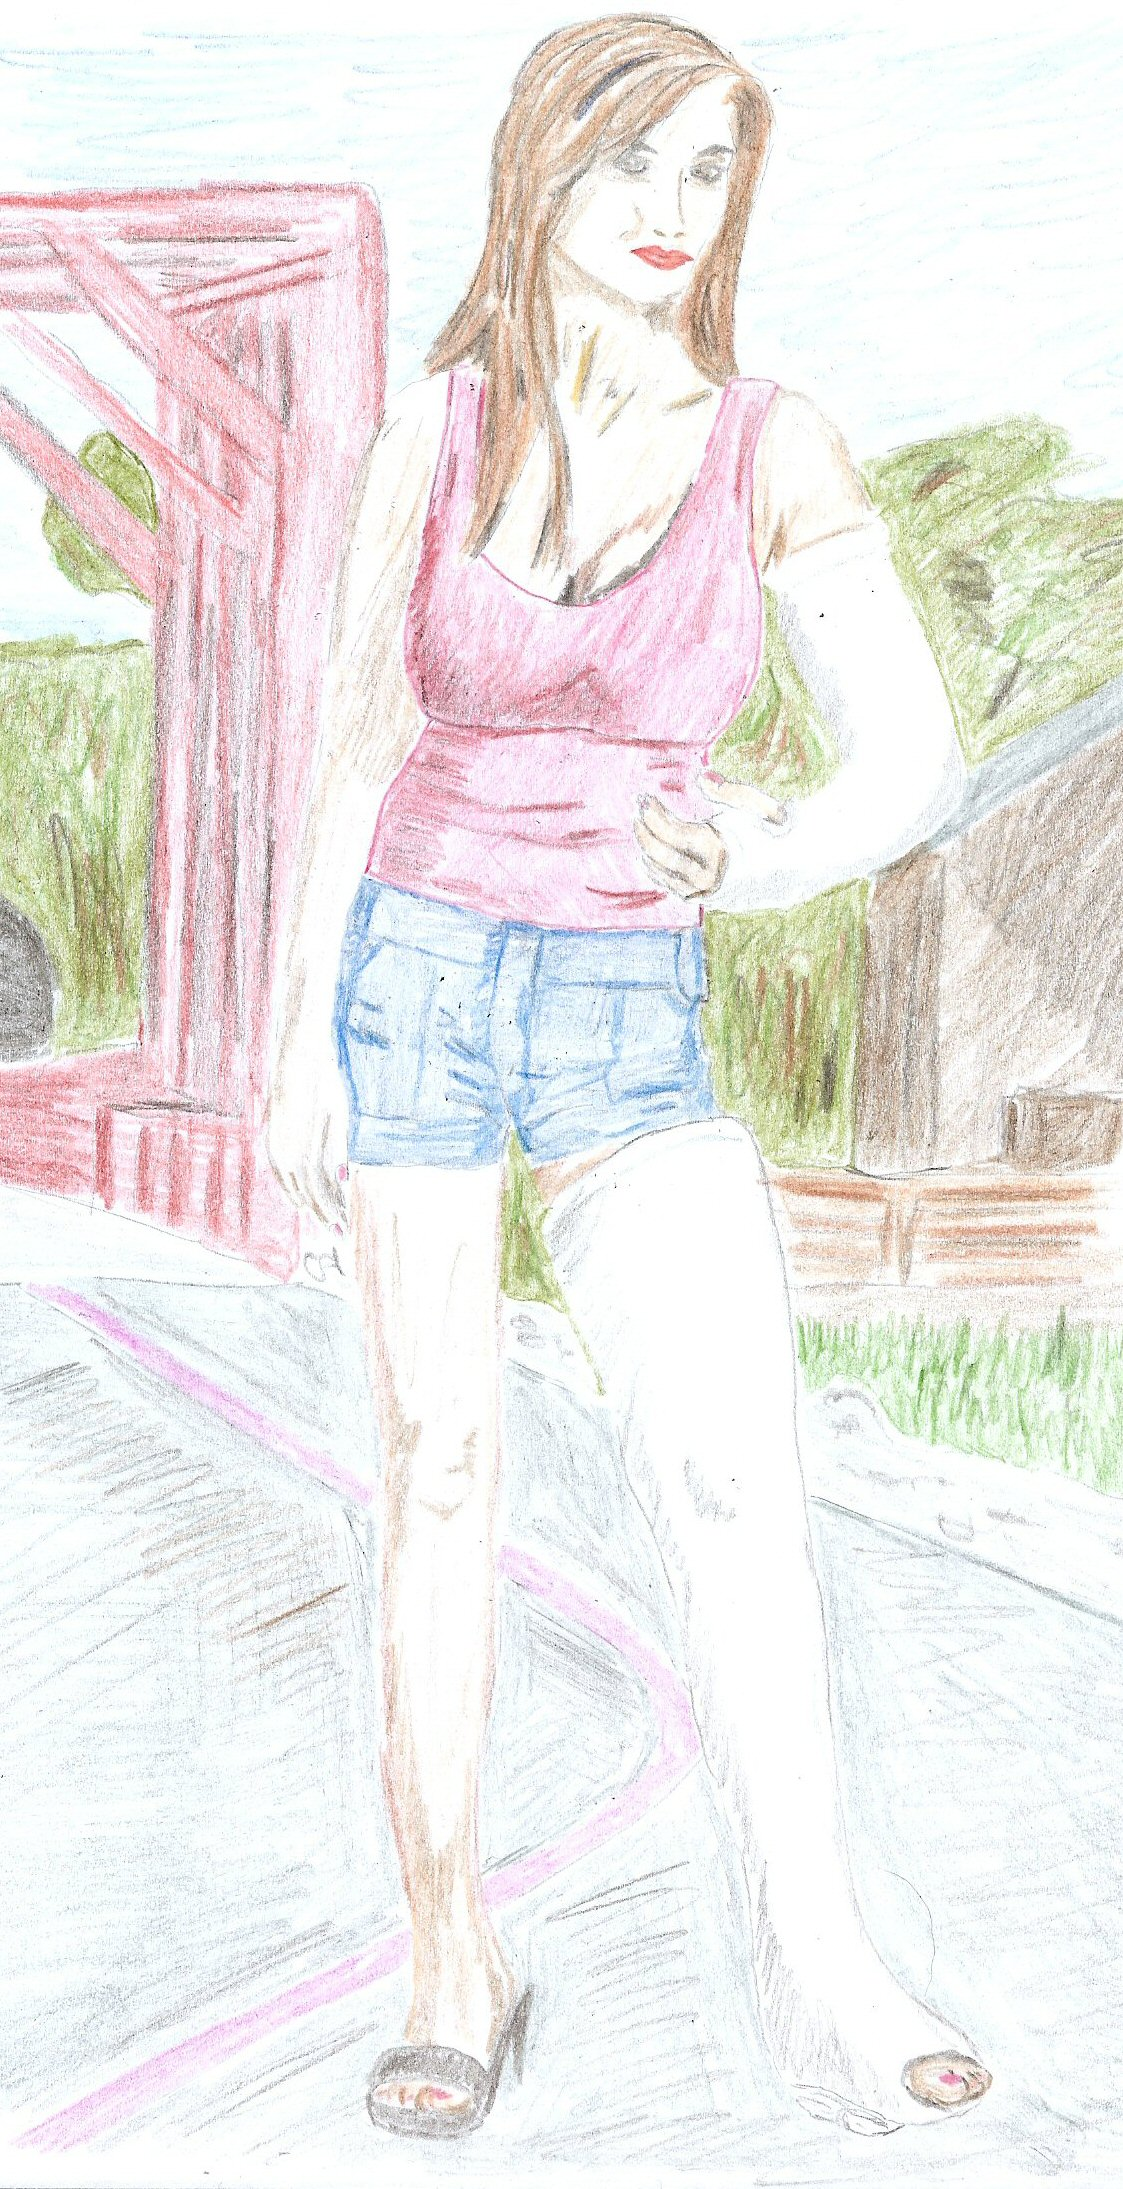
\includegraphics[height=\textheight]{images/kicks38.jpg}
\end{center}
